\documentclass[pagesize=auto, fontsize=11pt, DIV=11]{scrartcl}

%\usepackage{fixltx2e}
\usepackage{etex}
\usepackage{xspace}
\usepackage{lmodern}
\usepackage[T1]{fontenc}
\usepackage{textcomp}
\usepackage[svgnames]{xcolor}
\usepackage{listings}
\usepackage{microtype}
\usepackage{hyperref}
\usepackage{graphicx}
\usepackage{outline}
\usepackage{subcaption}
\usepackage{verbatim}
\usepackage{enumitem}
\usepackage{courier}
%\definecolor{backgroundColour}{gray}{0.90}
\definecolor{backgroundColour}{rgb}{0.95,0.95,0.92}

\lstdefinestyle{CStyle}{
    backgroundcolor=\color{backgroundColour},
    commentstyle=\color{Green},
    keywordstyle=\color{Blue},
    numberstyle=\tiny\color{Gray},
    stringstyle=\color{Purple},
    basicstyle=\footnotesize,
    breakatwhitespace=false,
    breaklines=true,
    captionpos=b,
    keepspaces=true,
    numbers=left,
    numbersep=10pt,
    showspaces=false,
    showstringspaces=false,
    showtabs=false,
    tabsize=2,                          % sets default tabsize to 2 spaces
    frame=single,                       % adds a frame around the code
    rulecolor=\color{black},
    language=C
}


\newcommand*{\mail}[1]{\href{mailto:#1}{\texttt{#1}}}
\newcommand*{\pkg}[1]{\textsf{#1}}
\newcommand*{\cs}[1]{\texttt{\textbackslash#1}}
\makeatletter
\newcommand*{\cmd}[1]{\cs{\expandafter\@gobble\string#1}}
\makeatother
\newcommand*{\env}[1]{\texttt{#1}}

\addtokomafont{title}{\rmfamily}

\lstset{%
  language=[LaTeX]TeX,%
  columns=flexible,%
  upquote=true,%
  numbers=left,%
  basicstyle=\ttfamily,%
  keywordstyle=\color{Navy},%
  commentstyle=\color{DimGray},%
  stringstyle=\color{SeaGreen},%
  numberstyle=\scriptsize\color{SlateGray}%
}

\title{MPI Shared Memory Programming}
\subtitle{User guide Draft}
\author{%
  Edgar F. Black\thanks{University of Illinois, Department of Computer Science, \mail{efblack2@illinois.edu}}%
  \and Luke Olson\thanks{\mail{lukeo@illinois.edu}}%
  \and William D. Gropp\thanks{\mail{wgropp@illinois.edu}}%
}
\date{DRAFT: \today} % Date

\begin{document}

\maketitle

\noindent


\begin{comment}

\begin{quote}
  \footnotesize
  The guide will present methods and best practices for efficient use of shared memory in two different contexts: \textbf{hybrid programing} and \textbf{share memory programing}.
\end{quote}
\end{comment}


%%%%%%%%%%%%%%%%%%%%%%%%%%%%%%%%%%%%%%%%%%%%%%%%%%%%%%%%%%%%%%%%%%%%%%%%%%%%%%%
% INSERT REAL CONTENT HERE
%
\section{Introduction}
%Although 
The message passing interface (MPI) has been the predominant parallel programming model since the mid-1900. It constitutes the base of the \emph{distributed} programming model in which components located on networked computers communicate and coordinate their actions by passing messages. Contrastingly, in a \emph{shared-memory} programming model, parallel processes share a global memory address space that they read and write to asynchronously. 

Today's clusters often comprise many nodes connected by a fast network each having processors that contain multiple cores. The current trend in cluster architecture shows an increasing number of cores per node, but also a declining memory per core. In traditional MPI programming, when a process is run on each of the n cores, for performance efficiency the data is often replicated at each process causing the memory demands of the application to grow linearly with the number of processes. Fortunately, the hardware often supports direct memory loads and stores, so these cores can be programmed to share part of the node's memory, potentially improving performance by reducing memory motion and footprint\cite{UsingAdvancedMPI}. 



\subsection*{Programming for Multicore}

The evolution towards multicore architecture has also force a shift in the traditional use of the \emph{distributed} programming model, in which all the communication between processes is handled essentially by the send/receive family of MPI functions, towards approaches that combines message passing with shared-memory techniques, often called \textbf{hybrid programming}\cite{UsingAdvancedMPI}. In this hybrid model, the threads or processes within a node communicate directly with each other by sharing the node's memory, while the inter-node communication is indeed handled using the send/receive traditional approach. One of the most common choice (among many) for hybrid programming, combines MPI for communication across nodes and OpenMP to share memory within a node. This approach is often referred as MPI+OpenMP.

\medskip

The MPI-3 standard added several functions to allow processes that exist within a node to directly allocate and share the node's memory, in a way similar to OpenMP. This new MPI Shared Memory model (MPI$_{sm}$) allows another approach to hybrid programming in which, traditional MPI is still used for inter-node communication while MPI$_{sm}$ is used for the intra-node communication through shared memory. In this document, this hybrid model is denoted as MPI+MPI$_{sm}$ to distinguish it from MPI+OpenMP. Brinskiy\cite{brinskiy2015} affirms that MPI$_{sm}$ can be used to incrementally change existing MPI codes in order to accelerate communication between processes on the shared-memory nodes.

\medskip

This MPI Shared Memory model, if proven to be efficient, could in turn become a viable alternative to OpenMP as a shared memory programming model.
 
\medskip

The objective of this guide is to describe, via examples, the shared memory capabilities introduced by the MPI-3 standard, and to explore its viability in the context of both the \textbf{share memory programming model} and as a \textbf{hybrid programming model}.


\subsection*{Systems and Compilers used}

All the computer utilized in this study corresponds to systems having more than one socket (ccNUMA nodes). These kind of architecture is ubiquitous nowadays. On those systems all the memory is accessible by all the cores, however the memory is distributed between the sockets. The efficient programming of these systems requires awareness of issues such as memory effects and thread/process placement.


Three compilers were used in the results presented in the following sections: the GNU \textbf{gcc}  version 7.3.0 (OpenMP 4.5), the Intel \textbf{icc} version 18.0.1 (OpenMP 5.0) and the  PGI \textbf{pgcc} version 18.3 (OpenMP 4.0). For the MPI implementation used, \textbf{gcc} and the \textbf{pgi} compliers both use \textbf{open-mpi} while the \textbf{intel} compiler used it own mpi implementation.



\subsection*{Organization}


\medskip

The lessons learned during the development of this work will be remarked and commented in the coming sections. This document is organized as follows:

\begin{itemize} 
\item Section 2 describes a small set of functions and techniques required to use MPI$_{sm}$ as a shared memory and as hybrid programming model.

\item Section 3 describes some technical aspects that affects the performance of both MPI$_{sm}$ and OpenMP.

\item Section 4 presents and compare results of the Stream benchmark obtained using MPI$_{sm}$ and OpenMP.

\item Section 5 compares the performance of MPI$_{sm}$ and OpenMP.

\item Section 6 compares the performance of two hybrid programming models: MPI+MPI$_{sm}$ and MPI+OpenMP.

\item Section 7 list a set of pros and cons of MPI$_{sm}$ as a shared memory and as hybrid programming model.

\item Section 8 contains a summary and conclusions.


%\item Section 5 describe some additional functions and techniques required by hybrid programming. Additionally it compares two hybrid programming model: MPI+MPI$_{sm}$ and MPI+OpenMP.

\end{itemize}








\begin{comment}






Today's trend of having 
an increasing number of cores per CPU (computing component, socket,chip) have created the need for approaches that combines the best of this two programming models: 


Almost all chips are multicore these days


 into what is nowadays known as Hybrid programming models.


It describes parallelism between processes having separate memory space; 

a 


in contrast to 

\emph{thread} parallelism which provides a shared memory model within a process. 

OpenMP and Pthreads are common examples of the \emph{thread} parallelism model.




Scale of machines to come encourage the use of different programming models to address issues such as

\begin{itemize} 

\item Declining memory per core

\item Multiple threads/core

\item Load balance

\item Algorithmic issues


\end{itemize}
\end{comment}


              % for SECTION 1    in "introduction.tex"
\section{MPI Shared Memory (MPI$_{sm}$)}

The MPI-3 standard developed an interface that allow processes inside a node to share the nodes' memory utilizing the well established functionality of Remote Memory Access (RMA), and some recently introduced functions. This permits the implementation of a shared memory programming model within a strictly MPI paradigm. This section lists and briefly describes a minimum set functions and data types used in writing MPI$_{sm}$ programs. 
\medskip

Additionally, to successfully develop hybrid programming, in which traditional send/receive functionality is used to communicate information among nodes while intra-node communication is handled via shared-memory, it is necessary a mechanism to distinguish between processes that belong to a given node from processes belonging to different nodes. This section also describes a procedure to achieve this goal. 

%Refer to the examples in the following sections or the MPI standard for a more detailed description.

\medskip

A description of the basic data types and function required by applications using MPI$_{sm}$, and pseudo codes illustrating their use, follows. The description is not intended to be comprehensive and the reader should consult the MPI-3 standard\cite{MPI-3}  or \cite{UsingAdvancedMPI} for a more information.


\medskip

\subsubsection*{Memory Window Data Type}

The memory in a process that can be accessed by another process through the use of Remote Memory Access (RMA) routines is called a \emph{memory window}. MPI-3 expand the use of memory windows into a portable mechanism that allows direct access, trough the CPU load/store instructions, of a process's memory by other process in the same node. Therefore, to use MPI$_{sm}$ it is required to define memory windows.

\medskip

MPI defines a data type, \textbf{\texttt{MPI\_Win}}, to be used as a handle in order to create and destroy memory windows. In addition to the conventional RMA uses of this data type, MPI$_{sm}$ use the \textbf{\texttt{MPI\_Win}} data type to dynamically allocate portions of memory to be shared by processes within a node and also to free that shared memory when it is not longer needed.


\subsubsection*{Shared Memory Communicator}

Before being able to allocate shared memory, the processes belonging to the main communicator (\textbf{\texttt{MPI\_COMM\_WORLD}}) must be separated into sub-communicators of processes existing inside a single node (intracommunicator). This is achieved by using the \textbf{\texttt{MPI\_Comm\_split\_type()}} function.

 

\subsubsection*{Shared Memory Allocation}

Once the memory window and the sub-communicator of processes existing inside a single node have been created, they are used to allocate shared memory using the new \textbf{\texttt{MPI\_Win\_allocate\_shared()}} function. This function returns a process-local pointer containing the address of the shared memory allocated by the calling process. It is a collective function and, therefore, must be called by all the processes of the intracommunicator, although any number of processes can specify a memory size=0.

\subsubsection*{Shared Memory Address Query}

The shared memory address allocated by the \textbf{\texttt{MPI\_Win\_allocate\_shared()}} function is meaningful only to the calling process and should not be communicated. Therefore, the \textbf{\texttt{MPI\_Win\_shared\_query()}} function can be used to retrieve the local base address of the shared memory on other processors.


\subsubsection*{Synchronization Techniques}

This is a behavior that MPI$_{sm}$ models after RMA data transfers. There are two basic methods used by MPI to complete data transfers (meaning when the data is ready to be used by the receiving process): active and passive target synchronization. 

\medskip

Active synchronization involves the use of the \textbf{\texttt{MPI\_Win\_fence()}} function while passive synchronization use a combination of the \textbf{\texttt{MPI\_Win\_lock()}}, \textbf{\texttt{MPI\_Win\_sync()}},  \textbf{\texttt{MPI\_Barrier()}} and \textbf{\texttt{MPI\_Win\_unlock()}} functions. 

\medskip

Passive synchronization is regarded as an advanced technique and it has been shown to outperform active synchronization in simple tests\cite{Samfass_2016} \cite{brinskiy2015}. However, active synchronization (\textbf{\texttt{MPI\_Win\_fence()}}) is less verbose, and the performance differences with respect to passive synchronization seems to diminish as the amount of work done in the context of the synchronization increases.

\medskip

All the examples and results shown in this work used the passive synchronization scheme unless explicitly indicated otherwise. This decision was made not because passive synchronization seems to outperform active synchronization, but because it was considered simpler to migrate form passive to active synchronization for any user wanting to test both techniques.

\subsubsection*{Shared Memory Deallocation}
When the shared memory is not longer needed, the memory window associated with that shared memory is not needed either. Therefore a call to \textbf{\texttt{MPI\_Win\_free()}} will free both, the allocated shared memory and the memory window.


\subsubsection*{Pseudo Code for MPI$_{sm}$ programing}

Figure \ref{fig:PseudoCode1} summarize a basic sequence that can be used for the MPI$_{sm}$ programing mode. The more relevant aspects of the code will be highlighted next.

\medskip

In line 3 a variable of type \textbf{\texttt{MPI\_Win}} declared. In line 5 the \textbf{\texttt{MPI\_Comm\_split\_type()}} function creates an intranode communicator (\textbf{\texttt{sm\_comm}}). The local (nodal) size and ranks for the processors belonging to the intranode communicator are determined in lines 8 and 9.

\medskip

Shared memory is allocated within the \textbf{\texttt{if-else}} statement in lines 13 to 19. Since the the \textbf{\texttt{MPI\_Win\_allocate\_shared()}} function is a collective one, all the processors in the communicator must call it. However, in this example, only rank 0 is actually allocating memory (look at the first parameter of the \textbf{\texttt{MPI\_Win\_allocate\_shared()}} function in lines 14 and 17). 

\medskip

Once the \textbf{\texttt{if-else}} statement is executed, only one process (rank 0) has access to the allocated shared memory. In order for the other processes to access that shared memory, the function \textbf{\texttt{MPI\_Win\_shared\_query()}} can be used to retrieve the local base addresses of other processes, as shown in line 22. (Strictly speaking, in this example, rank 0 don't need to call this function.) In calling this function, the second parameter is an integer corresponding to rank, within the intranode communicator, of the processor that allocated the shared memory. In our example this rank is 0. However, the MPI standard provides a predefined constant (\textbf{\texttt{MPI\_PROC\_NULL}}) that when used as the rank, returns the base address of the first process that specified a memory size greater than 0. Once this function returns, the variable \textbf{\texttt{sz}} will contain the size, in bytes, of the shared memory segment, while the variable \textbf{\texttt{dispUnit}} will contain the size, in bytes, of the basic type used in the allocation (4 bytes for float, 8 bytes for double etc.).


\medskip

Between lines 25 and 31 a passive synchronization access epoch is defined by the pair  \textbf{\texttt{MPI\_Win\_lock\_all}} and \textbf{\texttt{MPI\_Win\_unlock\_all}} functions for all processes sharing an RMA window.

\medskip

In line 26 a function is called to initialize the shared memory. In line 27 and 28, just before the shared memory can be utilized after initialization, calls to the \textbf{\texttt{MPI\_Win\_sync()}} function ensure completion of memory updates and then the \textbf{\texttt{MPI\_Barrirer()}} synchronize all processes on the node. That sequence must be repeated every time the shared memory buffer is modified and before it can be safely used.


\medskip

Finally, line 31 finish the passive synchronization access epoch, and line 34 free both, the allocated shared memory and the memory window.


\subsubsection*{Pseudo Code to for hybrid programing}

As mentioned earlier in this section, a hybrid program need a way to distinguish between processes that belong to a given node from processes belonging to different nodes. To accomplish this goal, the \textbf{\texttt{MPI\_Group\_translate\_ranks()}} function can be used as explained next, using Figure \ref{fig:PseudoCode2}.
 

\medskip

Lines 3 to 5 defines the global ranks and size of the \textbf{\texttt{MPI\_COMM\_WORLD}} communicator. In lines 7 and 8 an intranode communicator (\textbf{\texttt{sm\_comm}}) is created. Lines 10 and 11 define the local ranks within the intranode communicator.

\medskip

Lines 13 to 15 defines two MPI groups, one using the global and the other using the intranode communicators. Lines 17 to 19 declares and allocate two integer pointers (globalRank, localRank) each with a size equal to the size of global communicator. In lines 21 to 22 one of these pointers is initialized with as sequence representing the rank ids of global communicator.

\medskip

In line 24 the \textbf{\texttt{MPI\_Group\_translate\_ranks()}} function is called. This function requires as an input the global and local MPI groups created in lines 13 to 15, the integer array initialized in lines 21 to 22 (globalRank) and the size of the global communicator (worldSize). 

\medskip

The \textbf{\texttt{MPI\_Group\_translate\_ranks()}} function returns its output in the in the second pointer allocated in lines 17-19 (localRank). In general, the function sets the whole array to a predefined MPI integer constant (\textbf{\texttt{MPI\_UNDEFINED}}) except on the positions corresponding to processes belonging to the same node. 

\medskip

For example, running this code in four nodes, each having tree processes (for a total of 12 processes), after calling \textbf{\texttt{MPI\_Group\_translate\_ranks()}}, the content of the localRank array inside the processor having a worldRank equal to 7 (which corresponds to local rank 1 in node 2) is \emph{undefined} everywhere except in positions 6 to 8. The values in positions 6 to 8 corresponds to the local rank id for that node (0 to 2).


\medskip

With the information provided by the localRank pointer, it is easy to distinguish processes that belong to the same node from processes that exist elsewhere.


%\newpage

\begin{figure} [t!]
\centering
\captionsetup{justification=centering, singlelinecheck=false}
    
\begin{lstlisting}[style=CStyle]
int main(int argc, char *argv[])
{
    MPI_Win smWin;
    MPI_Comm sm_comm;
    MPI_Comm_split_type(MPI_COMM_WORLD,MPI_COMM_TYPE_SHARED, 0,MPI_INFO_NULL, &sm_comm);
    .
    int mySharedRank, sharedSize;
    MPI_Comm_rank(sm_comm,&mySharedRank);
    MPI_Comm_size(sm_comm,&sharedSize);
    .
    double *a;
    int size=1000;
    if (mySharedRank == 0) {
        MPI_Win_allocate_shared((MPI_Aint) size*sizeof(double), sizeof(double),MPI_INFO_NULL,
                                                 sm_comm, &a, &smWin);
    } else {
        MPI_Win_allocate_shared((MPI_Aint) 0                 , sizeof(double),MPI_INFO_NULL,
                                                 sm_comm, &a, &smWin);
    } // end if //                            
    MPI_Aint sz;
    int dispUnit;
    MPI_Win_shared_query(smWin, MPI_PROC_NULL, &sz,&dispUnit,&a);
    .
    .
    MPI_Win_lock_all(0,smWin);
   initialize(a,size);
    MPI_Win_sync(smWin);
    MPI_Barrier(sm_comm);
    .
    .
    MPI_Win_unlock_all(smWin);
    .
    .
    MPI_Win_free(&smWin);
    
    return 0;
} // end main() //
\end{lstlisting}    
\caption{Pseudo code for a basic MPI$_{sm}$ application.}
\label{fig:PseudoCode1}
\end{figure}


\begin{figure} [t!]
\centering
\captionsetup{justification=centering, singlelinecheck=false}
\begin{lstlisting}[style=CStyle]
int main(int argc, char *argv[])
{
    int myWorldRank, worldSize;
    MPI_Comm_rank(MPI_COMM_WORLD,&myWorldRank);
    MPI_Comm_size(MPI_COMM_WORLD,&worldSize);
    
    MPI_Comm sm_comm;
    MPI_Comm_split_type(MPI_COMM_WORLD,MPI_COMM_TYPE_SHARED, 0,MPI_INFO_NULL, &sm_comm);

    int mySharedRank;
    MPI_Comm_rank(sm_comm,&mySharedRank);

    MPI_Group sharedGroup,worldGroup;
    MPI_Comm_group(MPI_COMM_WORLD, &worldGroup);
    MPI_Comm_group(sm_comm, &sharedGroup);
    
    int *globalRank, *localRank;
    globalRank = (int *) malloc( worldSize * sizeof(int) );
    localRank  = (int *) malloc( worldSize * sizeof(int) );
    
    for (int i=0; i<worldSize; ++i) 
        globalRank[i]=i;

    MPI_Group_translate_ranks(worldGroup, worldSize, globalRank, sharedGroup, localRank);
    .
    .
    free(globalRank);
    free(localRank);
    .
    .
    MPI_Finalize();
    return 0;
} // end main() //
\end{lstlisting}    
\caption{Pseudo code for basic hybrid application.}
\label{fig:PseudoCode2}
\end{figure}





\begin{comment}

\begin{outline}
    \item {\bf MPI functions for shared memory }\\
      Description and use of the most relevant functions for shared memory introduced in MPI-3
    \item {\bf Shared Memory Allocation} \\
    Contiguous versus Noncontiguous memory allocation schemes\\
    Advantages and disadvantages\\
    Recommendations
    \item {\bf Relationship to Remote Memory Access }
      \begin{outline}
        \item {\bf Remote Memory Access Windows}
      \end{outline}
    \item {\bf Synchronization Techniques} \\
    Difference between $\textbf{MPI\_Win\_fence()}$ and $\textbf{MPI\_Win\_sync()}$

\end{outline}

\end{comment}

                    % for SECTION 2    in "mpi_sm.tex"
\section{Memory bandwidth and Barriers as limits in shared memory programing models}

In this section two technical aspects that can potentially affect the overall performance of applications conforming to the shared memory programing model are evaluated. The first is related to the performance of the computer's memory sub-system, and the second relates to the cost of the barriers required by parallel program to ensure correct results.
%\medskip


\subsection*{Stream Benchmark}

For a long time we have witness how CPUs are being getting faster much more quickly than the computer's memory sub-system. Modern multi-core processors have become voracious consumers of data, and, as a consequence, more and more programs are being limited in performance by the memory bandwidth of the system, rather than by the computational performance of the CPU\cite{McCalpin2007}. It is, therefore, particularly important to be able to determine the memory bandwidth of the system at hand. 

\medskip


The STREAM benchmark\cite{McCalpin2007} is a suite of four (Copy, Scale, Add and Triad) simple tests that measures sustainable memory bandwidth (in MB/s) and the corresponding computation rate for simple vector kernels. In general, it is used to measure the evolution of the memory bandwidth of shared memory systems as more computing component are included in the test. Traditionally, the test has been implemented using OpenMP and the computing component are usually referred as threads.

\medskip

For MPI$_{sm}$ to become a viable alternative to OpenMP in the context of the shared memory programing model, it is fundamental that its sustainable memory bandwidth compares favorably to its OpenMP counterpart.

\medskip

The stream program that can be download from its web site \cite{McCalpin2007} is already annotated with directives (\textbf{\#pragma}) to make it a correct OpenMP program. This program was modified in order to develop an equivalent  MPI$_{sm}$ version. Both programs were run, using various compilers and MPI implementations. Some results, as well as lessons learned, follow.

\medskip

Figure \ref{fig:TriadTestBefore} presents results obtained on one system (\textbf{stout}) for the Triad test of the stream suite; results of the other tests (Copy, Scale and Add) are similar. The left plot, (\ref{fig:TriadBefore}) shows the actual bandwidth achieved while the right plot (\ref{fig:TriadRatioBefore}) show the MPI$_{sm}$ to OpenMP ratio obtained.
 
\medskip

\begin{figure} [h!]
    \centering
    \captionsetup{justification=centering, singlelinecheck=false}
    \begin{subfigure}{.6\textwidth}
      \hspace*{-1.5cm} 
      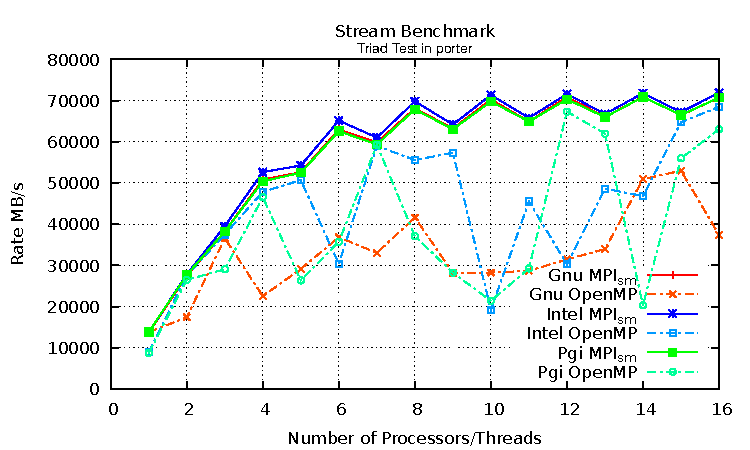
\includegraphics[width=0.95\linewidth]{Plots/streamBenchmark/porter-TriadBefore.pdf}
      \caption[]{Bandwidth per number of processes/threads.}
      \label{fig:TriadBefore}
    \end{subfigure}%
    \begin{subfigure}{.6\textwidth}
      \hspace*{-1.5cm} 
      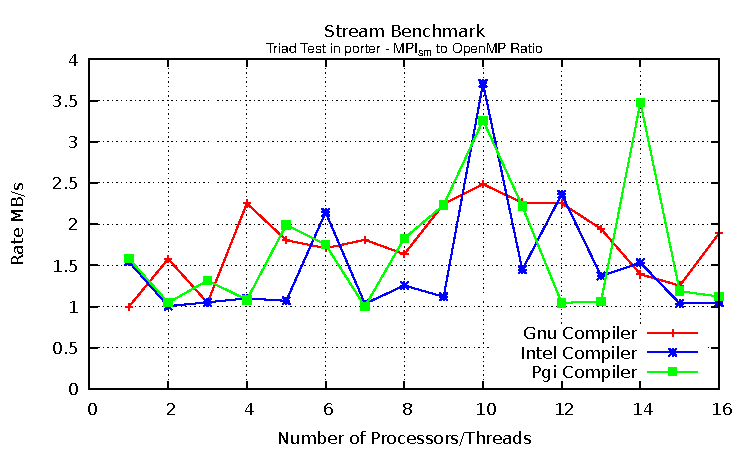
\includegraphics[width=0.95\linewidth]{Plots/streamBenchmark/porter-TriadRatioBefore.pdf}
      \caption{Ratio MPI$_{sm}$ to OpenMP.}
      \label{fig:TriadRatioBefore}
    \end{subfigure}
    \caption{Triad test. No binding policy for OpenMP}
\label{fig:TriadTestBefore}
\end{figure}


In Figure \ref{fig:TriadBefore} the segmented lines correspond to OpenMP while the continuous lines represent MPI$_{sm}$. Notice the extremely irregular behavior shown by all the OpenMP cases. Exploring the causes of such behavior lead to the first lesson in this section: \textbf{thread placement}. As mentioned in the Introduction, all the systems used in this study corresponds to systems having more than one socket. In this kind of systems, application having multiple threads could run into affinity problems.

\medskip

The lack of a \emph{by-default} thread affinity control policy of all the compilers used in the study results the erratic behavior shown in the Figure \ref{fig:TriadBefore}, because the threads are allow to be moved, by the OS, not only to a different core but also to a different socket. On the other hand, the more stable behavior that can be observed for the MPI$_{sm}$ case is due to the fact that the MPI implementations used \emph{do} have a \emph{by-default} binding policy for the processes running in the node.

\medskip

The ways to control thread affinity in OpenMP used to be compiler-dependent. However, OpenMP version 4.0 specification introduced a standardized mean to control thread affinity allowing, for the first time, an uniform way to have fine grain control over the affinity policy to compilers conforming to the standard. It introduced two new concepts: binding policy and place partition.

The binding policy determines if the threads will be bound and how they will be distributed, while the place partition is the set of places to which threads can be bound. One simple way of control the binding policy is by setting the \textbf{\texttt{OMP\_PROC\_BIND}} environment variable. Similarly, a way of control the place partition is by setting the \textbf{\texttt{OMP\_PLACES}} environment variable. 

\medskip

In our case, we found convenient to set 

\begin{itemize} 

\item \textbf{\texttt{OMP\_PROC\_BIND}}=spread 

\item \textbf{\texttt{OMP\_PLACES}}=sockets

\end{itemize}

meaning that the threads will be bound and distributed (or spread) among the sockets. More details about the values allowed for these enviromantal variables can be found in the current OpenMP API specification.

\medskip

Once a thread policy was set for the OpenMP cases, the stream tests were run again and the results are shown in Figure \ref{fig:TriadTest}. As before, the left plot, (\ref{fig:Triad}) shows the actual bandwidth achieved while the right plot (\ref{fig:TriadRatio}) show the MPI$_{sm}$ to OpenMP ratio obtained. 

\medskip
From the results shown in Figure \ref{fig:TriadTest} it can be seen that the sustainable memory bandwidth achievable by MPI$_{sm}$ is effectively at pair with its OpenMP counterpart.


\begin{figure} [h!]
    \centering
    \captionsetup{justification=centering, singlelinecheck=false}
    \begin{subfigure}{.6\textwidth}
      \hspace*{-1.5cm} 
      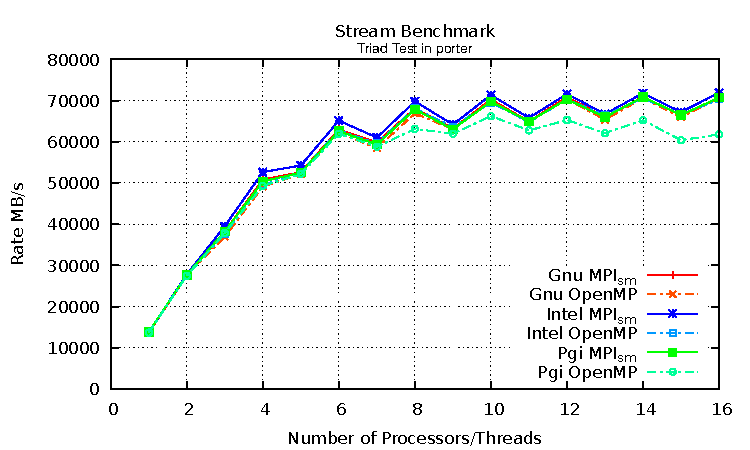
\includegraphics[width=0.95\linewidth]{Plots/streamBenchmark/porter-Triad.pdf}
      \caption[]{Bandwidth per number of processes/threads.}
      \label{fig:Triad}
    \end{subfigure}%
    \begin{subfigure}{.6\textwidth}
      \hspace*{-1.5cm} 
      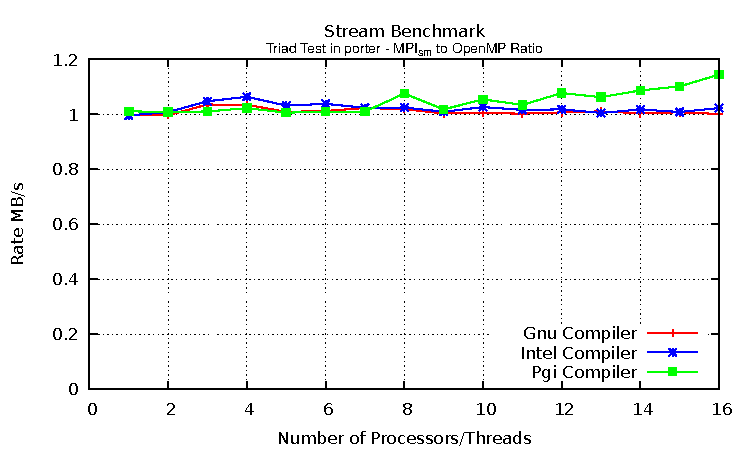
\includegraphics[width=0.95\linewidth]{Plots/streamBenchmark/porter-TriadRatio.pdf}
      \caption{Ratio MPI$_{sm}$ to OpenMP.}
      \label{fig:TriadRatio}
    \end{subfigure}
\caption{Triad test.}
\label{fig:TriadTest}
\end{figure}

\newpage

\subsection*{Barriers}
%causes a central processing unit (CPU) or compiler to enforce 

A memory barrier is a type of instruction that requires an ordering constraint on memory operations issued before and after it. They are necessary because most modern CPUs employ performance optimizations that can result in out-of-order execution. This reordering of memory operations (loads and stores) can produce incorrect results in parallel programs unless carefully controlled.

\medskip

The efficiency of the barrier implementation could potentially affect the overall performance of parallel applications conforming to the shared memory programing model. Therefore an effort was made to estimate, as accurate as possible, the time delay produced by the barrier itself, because a large difference in this delay between MPI$_{sm}$ and OpenMP could result crucial in choosing one or the other.

\medskip


Notice that what is being measured is not the time a particular thread/process wait in the barrier, which, in general, depends on the load unbalance; e.g. the time a thread/process is in the barrier waiting for its partners to arrive. However, the parameter being measured could be approximated by the minimum, among all the thread/process of the
time just described.




\medskip


\begin{figure} [h!]
\centering
\captionsetup{justification=centering, singlelinecheck=false}
    
\begin{lstlisting}[style=CStyle]
for (uint64_t n=0 ; n<max_iterations; ++n) {

    MPI_Barrier(sm_comm);
        
    clock_gettime(CLOCK_MONOTONIC, &start);
    MPI_Barrier(sm_comm);    
    clock_gettime(CLOCK_MONOTONIC, &end);
    
    diff = BILLION * (end.tv_sec - start.tv_sec) + end.tv_nsec - start.tv_nsec;
    MPI_Allreduce( MPI_IN_PLACE, &diff, 1, MPI_UNSIGNED_LONG, MPI_MIN,sm_comm);
    barrier_time+=diff;

}	// end for //
\end{lstlisting}    
\caption{Pseudo used to estimate MPI$_{sm}$ barrier time.}
\label{fig:PseudoCode3}
\end{figure}


\medskip


\begin{figure} [h!]
    \centering
    \captionsetup{justification=centering, singlelinecheck=false}
    \begin{subfigure}{.6\textwidth}
      \hspace*{-1.5cm} 
      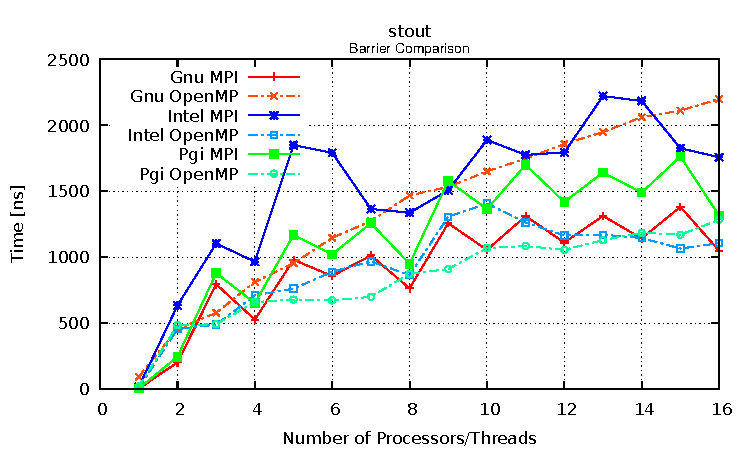
\includegraphics[width=0.95\linewidth]{Plots/barrier/stout.pdf}
      \caption[]{Estimated time.}
      \label{fig:Barrier}
    \end{subfigure}%
    \begin{subfigure}{.6\textwidth}
      \hspace*{-1.5cm} 
      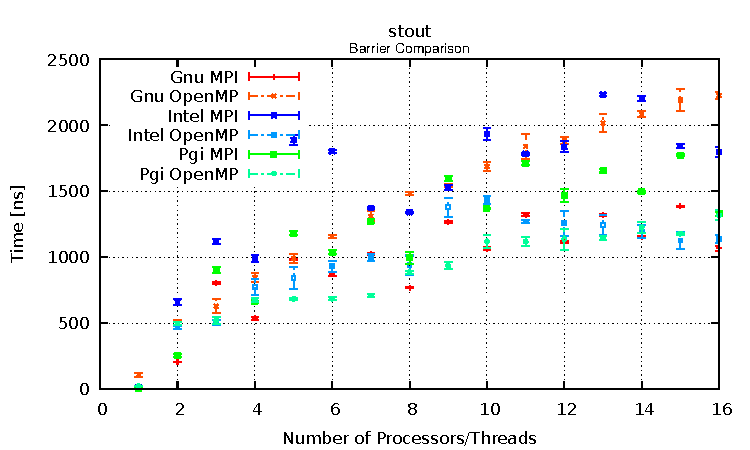
\includegraphics[width=0.95\linewidth]{Plots/barrier/stoutError.pdf}
      \caption{Errorbars to show variability of results.}
      \label{fig:BarrierErrorBars}
    \end{subfigure}
\caption{Barrier Results.}
\label{fig:BarrierAndErrorBars}
\end{figure}





\begin{comment}


Two identical versions of the stream benchmarks one using  and 
 were created and it 
 results are compared below for several systems. 
 
 
 However, the arrays 



 capabilities of the 

an MPI$_{sm}$ version of the program was developed and used to compare its performance to that obtained using its 



OpenMP versions of the STREAM benchmark program has been used to measure the evolution of the sustainable memory bandwidth of shared memory system as more threads are included in the test. 




What is STREAM?
The STREAM benchmark is a simple synthetic benchmark program that measures sustainable memory bandwidth (in MB/s) and the corresponding computation rate for simple vector kernels. 

Why should I care?

Computer cpus are getting faster much more quickly than computer memory systems. 

As this progresses, 

As an extreme example, several current high-end machines run simple arithmetic kernels for out-of-cache operands at 4-5 percent of their rated peak speeds --- that means that they are spending 95-96 percent of their time idle and waiting for cache misses to be satisfied.

The STREAM benchmark is specifically designed to work with datasets much larger than the available cache on any given system, so that the results are (presumably) more indicative of the performance of very large, vector style applications.

If you want more words, I have written a paper on STREAM: Sustainable Memory Bandwidth in Current High Performance Computers

A somewhat broader look on the issue, see my paper: Memory Bandwidth and Machine Balance in Current High Performance Computers. STREAM is also a useful component of models for scaling of homogeneous throughput workloads (like the SPEC CPU "rate" benchmarks). 

Examples of models based on STREAM measurements that do a pretty good job of estimating SPECfp rate2000 scaling are included in several presentations.

\end{comment}

           % for SECTION 3    in "streamBenchmark.tex"
%\section{Share Memory Programing}

In this section two computer programs are used to evaluate the performance of the MPI$_{sm}$ by comparing it to equivalent versions of the programs developed using OpenMP. The objective is to test the capabilities of MPI$_{sm}$ as a shared memory programing model and to evaluate its viability as an alternative to OpenMP.


\subsection*{Jacobi iteration}
The first program consists of a Jacobi iteration, solving the 2D-Laplace equation, a common technique to approximate the solution of elliptic PDEs within some allowable tolerance. Results form two versions (MPI$_{sm}$ vs OpenMP) of the program are compared below. The two versions of this program were later modified into hybrid versions. Results for the hybrid cases are presented in section 5.

Figure \ref{fig:Figure1} presents results from the Jacobi iteration program. This results were obtained in \emph{dunkel}; a computer having an Intel(R) Xeon(R) CPU E5-2650 v4 running at 2.20GHz. The plot in the left (Figure \ref{fig:RatioDunkel}) shows the ratio between the time taken by the MPI$_{sm}$ to the OpenMP versions of this program as a function of the number of threads/processors used, while the plot in the right (Figure \ref{fig:TimeDunkel}) shows actual execution time.


\begin{figure} [h!]
    \centering
    \captionsetup{justification=raggedright, singlelinecheck=false}
    \begin{subfigure}{.6\textwidth}
      \hspace*{-1.5cm} 
      \includegraphics[width=0.95\linewidth]{Plots/section3.1/dunkelRatio.pdf}
      \caption[]{Jacobi iteration - Ratio MPI$_{sm}$ to OpenMP.}
      \label{fig:RatioDunkel}
    \end{subfigure}%
    \begin{subfigure}{.6\textwidth}
      \hspace*{-1.5cm} 
      \includegraphics[width=0.95\linewidth]{Plots/section3.1/dunkel.pdf}
      \caption{Jacobi iteration - Execution time}
      \label{fig:TimeDunkel}
    \end{subfigure}
\caption{Comparing shared memory programing models - Jacobi iteration in dunkel}
\label{fig:Figure1}
\end{figure}

Figure \ref{fig:Figure2} presents similar results obtained in one node of \emph{Blue Waters}. In this case the CPU is an AMD Opteron(TM) Processor 6276 running at 2.30GHz. 

\begin{figure} [h!]
    \centering
    \captionsetup{justification=raggedright, singlelinecheck=false}
    \begin{subfigure}{.6\textwidth}
      \hspace*{-1.5cm} 
      \includegraphics[width=0.95\linewidth]{Plots/section3.1/blueWatersRatio.pdf}
      \caption{Jacobi iteration - Ratio MPI$_{sm}$ to OpenMP.}
      \label{fig:RatioBW}
    \end{subfigure}%
    \begin{subfigure}{.6\textwidth}
      \hspace*{-1.5cm} 
      \includegraphics[width=0.95\linewidth]{Plots/section3.1/blueWaters.pdf}
      \caption{Jacobi iteration - Execution time}
      \label{fig:TimeBW}
    \end{subfigure}
\caption{Comparing shared memory programing models - Jacobi iteration in one \emph{Blue Waters} Node}
\label{fig:Figure2}
\end{figure}

\medskip


Figures \ref{fig:RatioDunkel} and \ref{fig:RatioBW} express the ratio of time taken by MPI$_{sm}$ to OpenMP to solve the same problem using the same number of iterations. While for \emph{dunkel} this ratio approach 0.5 as the number of processors/threads increases (meaning that MPI$_{sm}$ takes about half ot the time taken by OpenMP), for one node of \emph{Blue Waters} this ratio was close to 1.0 and independent of the number of processors/threads used in the solution.

\medskip

Figures \ref{fig:TimeDunkel} and \ref{fig:TimeBW} are shown here to provide a perspective of the time taken to achieve the solution. Every point shown in these plots correspond to the minimum time collected over 5 runs.
\medskip



\subsection*{Computational Fluid Dynamic}
The second program used to compare these share memory programing models consists of a 3D Computational Fluid Dynamic (CFD) parallel program. The original version of the program was written in OpenMP. The program was modified to create an MPI$_{sm}$ version. The results shown corresponds to solutions using double precision arithmetics. 

\medskip

Figure \ref{fig:Figure3} and \ref{fig:Figure4} presents results from the CFD program. This results were obtained in the same computers used for the Jacobi iteration case. Once again, the plots in the left side shows the ratio between the time taken by the MPI$_{sm}$ to the OpenMP versions of this program as a function of the number of threads/processors used (a ratio grater than one means that MPI$_{sm}$ takes more time than OpenMP to produce a solution), while the plot in the right shows actual execution time.



\begin{figure} [h!]
    \centering
    \captionsetup{justification=raggedright, singlelinecheck=false}
    \begin{subfigure}{.6\textwidth}
      \hspace*{-1.5cm} 
      \includegraphics[width=0.95\linewidth]{Plots/section3.2/dunkelDPRatio.pdf}
      \caption{Computational Fluid Dynamic - Ratio MPI$_{sm}$ to OpenMP.}
      \label{fig:RatioDunkelCFD}
    \end{subfigure}%
    \begin{subfigure}{.6\textwidth}
      \hspace*{-1.5cm} 
      \includegraphics[width=0.95\linewidth]{Plots/section3.2/dunkelDP.pdf}
      \caption{Computational Fluid Dynamic - Execution time}
      \label{fig:TimeDunkelCFD}
    \end{subfigure}
\caption{Comparing shared memory programing models - CFD in \emph{dunkel}}
\label{fig:Figure3}
\end{figure}

\medskip


\begin{figure} [h!]
    \centering
    \captionsetup{justification=raggedright, singlelinecheck=false}
    \begin{subfigure}{.6\textwidth}
      \hspace*{-1.5cm} 
      \includegraphics[width=0.95\linewidth]{Plots/section3.2/blueWatersDPRatio.pdf}
      \caption{Computational Fluid Dynamic - Ratio MPI$_{sm}$ to OpenMP.}
      \label{fig:RatioBWCFD}
    \end{subfigure}%
    \begin{subfigure}{.6\textwidth}
      \hspace*{-1.5cm} 
      \includegraphics[width=0.95\linewidth]{Plots/section3.2/blueWatersDP.pdf}
      \caption{Computational Fluid Dynamic - Execution time}
      \label{fig:TimeBWCFD}
    \end{subfigure}
\caption{Comparing shared memory programing models - CFD in one \emph{Blue Waters} Node}
\label{fig:Figure4}
\end{figure}



For the CFD case, Figures \ref{fig:RatioDunkelCFD} and \ref{fig:RatioBWCFD}, presenting the ratio of time taken by MPI$_{sm}$ to OpenMP, show results that contrast with the ones obtained for the Jacobi iteration case. For both \emph{dunkel} and one node of \emph{Blue Waters}, this ratio is grater than one for two or more processes/threads and it has a tendency to increase as more processes/threads are added. This tendency to increase is more pronounced in \emph{Blue Waters} where this ratio grows to two for 12 processes/threads and still increases even more.

Once again, Figures \ref{fig:TimeDunkelCFD} and \ref{fig:TimeBWCFD} are shown here to provide a perspective of the time taken to achieve the solution. 

\medskip

\begin{comment}
\subsubsection*{Partial improvement using node topology}

Information about hardware threads, core, cache, socket topology can help to implement binding between cores and processes/threads. It is known that applications with frequent synchronization between "neighboring" processes/threads could profit from placing them close together. To test this idea, a simple tool called \emph{\textbf{taskset}} was used in \emph{dunkel} in a setting similar to the one used to produce Figure \ref{fig:Figure3}. This particular computer (\emph{dunkel}) has two sockets, each having 12 cores, for a total of 24 cores, each corresponding to the 24 processes/threads shown in Figures \ref{fig:Figure1} and \ref{fig:Figure3}. The 12 cores in one socket of \emph{dunkel} shared 30 Mbi of L3 cache. A new experiment was set to run within a single socket using the '-c 0-11' parameter of taskset. 

The results of this new experiment are shown in Figure \ref{fig:taskset}. Notice that only 12 processes/threads are uses. 

\medskip


\begin{figure} [h!]
    \centering
    \captionsetup{justification=raggedright, singlelinecheck=false}
    \begin{subfigure}{.6\textwidth}
      \hspace*{-1.5cm} 
      \includegraphics[width=0.95\linewidth]{Plots/section3.2/dunkel-DP-1SoketRatio.pdf}
      \caption{Computational Fluid Dynamic - Ratio MPI$_{sm}$ to OpenMP.}
      \label{fig:RatioDunkelCFD_Pin}
    \end{subfigure}%
    \begin{subfigure}{.6\textwidth}
      \hspace*{-1.5cm} 
      \includegraphics[width=0.95\linewidth]{Plots/section3.2/dunkel-DP-1Soket.pdf}
      \caption{Computational Fluid Dynamic - Execution time}
      \label{fig:TimeDunkelCFD_Pin}
    \end{subfigure}
\caption{Comparing shared memory programing models - CFD in \emph{dunkel}}
\label{fig:taskset}
\end{figure}

\medskip

Notice that the ratio of time taken by MPI$_{sm}$ to OpenMP, shown in Figure \ref{fig:RatioDunkelCFD_Pin} is close to 1 indicating a similar performance between the MPI$_{sm}$ and the OpenMP versions of the program.
...




%similar behavior 

%as the one shown in Figure \ref{fig:RatioDunkelCFD}, 

%that the ratio MPI$_{sm}$ to OpenMP is almost always grater than one, and increasing as more processes/threads are used in the solution up to a value close to 1.7.

\end{comment} 


\subsection*{Analysis}
The two cases presented in this section show conflicting results with respect to one shared memory programing model being better than the other. What is clear is that MPI$_{sm}$ can perform as good or better than OpenMP under the right conditions. To try to determine and understand what those condition are is part of what we are trying to accomplish.


   % for SECTION 4    in "share_memory_programing.tex"
%\section{Hybrid Programming} % using MPI+MPI$_{sm}$}

Most HPC systems in use today are clusters of shared memory nodes. The idea of hybrid programming consists of combining parallelization on the node interconnect with parallelization inside of each node. Traditionally, parallelization between nodes is being achieved using a distributed memory programming model such as MPI, while parallelization inside nodes is achieved using a shared memory programming model such as OpenMP, posix threads, or MPI$_{sm}$. 

\medskip
It has been recognized that getting good performance from a hybrid model can be difficult and requires understanding how the different programming models may interact \cite{UsingAdvancedMPI}. However, there are several reasons for using hybrid programing:

\begin{itemize} 

\item To reduce the memory footprint. Many codes require large lookup data structures that are global to the computation and ofter constant. For performance efficiency the data is ofter replicated at each process causing the memory demands of the application to grow with the number of processes. Sharing memory between MPI processes inside a node can often allow a way to share the data structure and keep only one copy per node instead of one copy per process. Nowadays this is becoming increasingly important since the number of cores in supercomputers is growing much faster than the number of nodes and than the amount of memory-per-core.

\item To reduce communication among processes. This could be achievable by directly accessing memory eliminating the need of communication through message passing between processes inside nodes.


\end{itemize}


\medskip

This section presents results of a parallel sparse matrix-vector multiplication (SPMV), a widely used operation in many simulations and the main kernel in iterative solvers, and compares its performance with and without using shared memory.


\medskip


\subsection*{Parallel SPMV}

The sparse matrix-vector multiplication (SPMV) consist in solving Equation (\ref{eq:spmv}), where A is a sparse \emph{N X N} matrix and \emph{v} is a dense \emph{N}-dimensional vector \cite{BienzGO16}.


\begin{equation}
  w = A * v
\label{eq:spmv}  
\end{equation}

In parallel, the sparse system is often distributed across processes such that each process holds a contiguous subset of rows from matrix \emph{A} and the corresponding subset of rows from vectors \emph{v} and \emph{w}. Within a single processes, it is common to splits the non-zeros values of its rows into two groups: an on-process block containing values associated to columns of the matrix that correspond to the part of vector \emph{v} values stored locally, and an off-process block containing the remainder of the non-zeros that are associated with vector \emph{v} values that are stored on other processes\cite{BienzGO16}. This is illustrated in Figure \ref{fig:Matrix}, for a case in which the matrix \emph{A} and vectors \emph{v}, \emph{w} are divided among four processes. Different colors are used to illustrate the on-process block corresponding to each process. The same color is used to show the corresponding part of vectors \emph{w} and \emph{v}. In each process the off-process values of \emph{A} occupy the remainder space, shown here without color.

\medskip

\begin{figure}[h!]
    \centering
    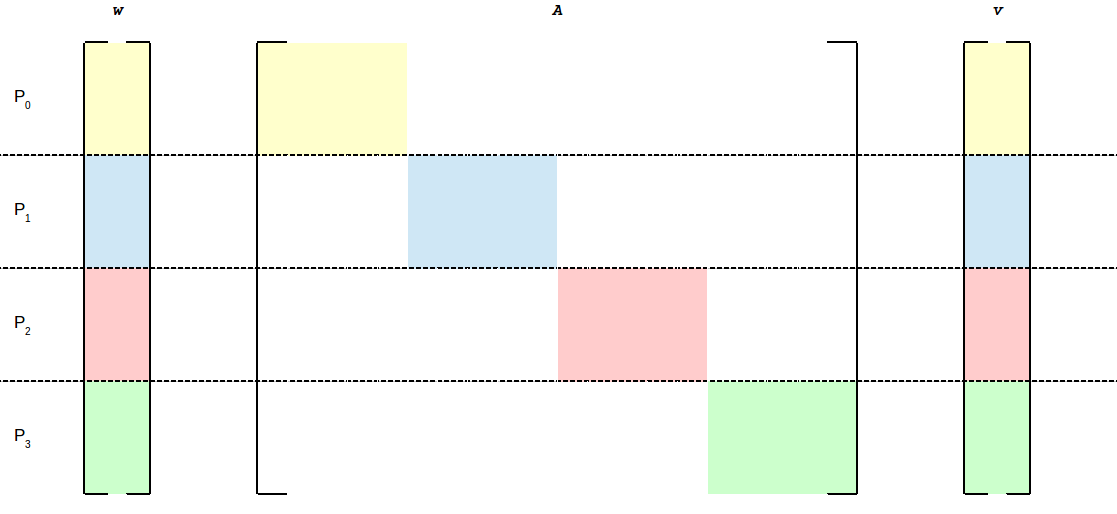
\includegraphics[width=100mm]{Plots/HybridProgramming/matrix.png}
    \caption{On-Proccess blocks shown in color.}
    \label{fig:Matrix}
\end{figure}

\medskip



With this configuration, the solution of Equation (\ref{eq:spmv}) can be obtained by executing it twice in each process. The first time using only the on-process block of matrix \emph{A} and the on-process part of the \emph{v} vector. The second time using the off-process block of matrix \emph{A} and elements of the \emph{v} vector held in other processes. These two partial solutions must be added to obtain the actual solution. Notice that while the first solution can be performed by each process independently, not requiring any communication among processes, the second solution require communication among the processes because each process requires part of the \emph{v} vector existing in other processes. For a more detailed explanation on the whole algorithm the reader could take a look at \cite{BienzGO16}.

\medskip

It is known that, as the number of processes increases, the communication time start to dominate the execution time of the kernel. This is true even when communication is carefully overlapped with communication. As stated above, the communication part of this process consist in receiving parts of the \emph{v} vector held in other processes. These parts need to be communicated, perhaps using traditional send/receive calls, even if both processes involved in the communication reside in the same node.

\medskip

The amount of communication of this kernel can be reduced if a process could have direct access to elements of the \emph{v} vector beyond those held by itself. One extreme way to achieve this is by replicating the whole \emph{v} vector in each process; that would eliminate all the required communication. However, given that the \emph{v} vector is dense, this is, in general, a prohibitive alternative. 

\medskip

Another possibility would be if all the processes residing inside a node could have direct access to the parts of the \emph{v} vector already existing in the node. Referring to Figure \ref{fig:Matrix}, assume a case in which first two processes resides in a node, $N_0$, while the last two processes resides in a different node, $N_1$. The parts of the \emph{v} vector corresponding to $P_0$ and $P_1$ are in $N_0$, but these parts are only accessible by their corresponding process. However, if these parts of the \emph{v} vector were allocated using shared memory, they would be accessed by all the processes in the node. 

\medskip

Figure \ref{fig:MatrixSm} help to illustrate the case of using shared memory for storing the \emph{v} vector. Here the shared memory is represented by the absence of separation in \emph{v} vector between the part held in $P_0$ and $P_1$ and between $P_2$ and $P_3$ as compared to Figure \ref{fig:Matrix}. Under this configuration, the processes inside a node (e.g. $P_0$ and $P_1$ in $N_0$) are able to access all the elements of the \emph{v} vector existing in that node. Additionally, the on-process block of matrix \emph{A} is expanded (and the off-process block contracted) proportionally to the number of processes existing in the node, effectively eliminating all the intra-node communication, and reducing the communication to only the inter-node part. Notice that all the part of matrix \emph{A} and of the \emph{w} vector belonging to a process are still completely hidden (not shared) form all the other processes.



\begin{figure}[t!]
    \centering
    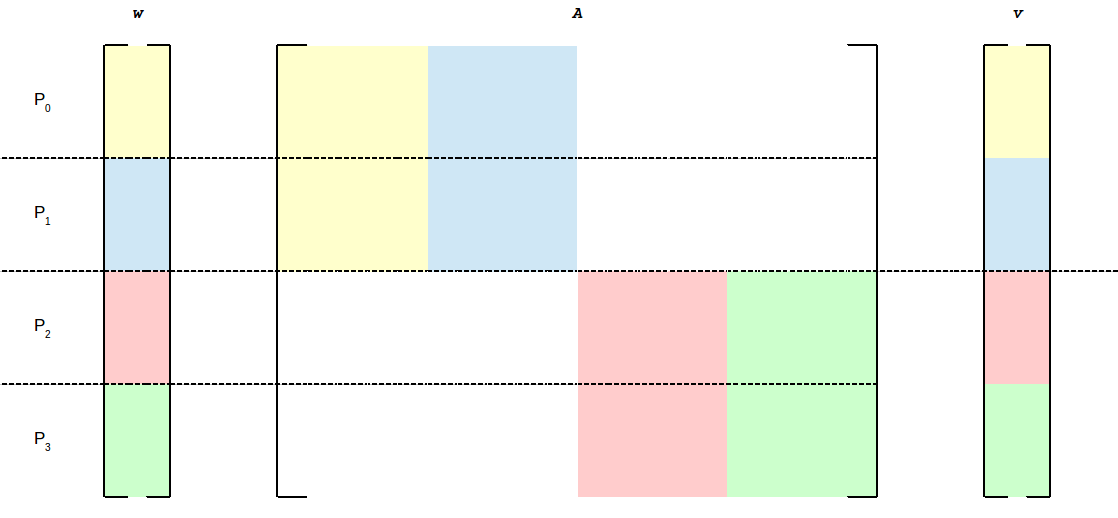
\includegraphics[width=100mm]{Plots/HybridProgramming/matrixSm.png}
    \caption{Expanded On-process blocks per process due to use of shared memory.}
    \label{fig:MatrixSm}
\end{figure}

\medskip

\subsection*{Preliminary Results}


The idea of using shared memory to reduce communication in the SPMV kernel, presented in the previous section,
was implemented in one of the SPMV functions inside Raptor, a high performance algebraic multigrid solver \cite{BiOl2017}. Preliminary results are presented in this section. 

\medskip

The following figures compare the performance of two the SPMV kernel implementations: one using traditional MPI and the other, a hybrid one, using the shared memory capabilities of MPI-3 ($MPI+MPI_{Sm}$).

\medskip

First, results obtained using individual systems (one node) are presented. For this case, all the communication among the processors is intra-node, and therefore is totally eliminated by the use of shared memory. Later, results obtained using a small 4-node cluster and Blue Waters are also presented.

\medskip

Figure \ref{fig:spmvIndividual} shows the results obtained in individual systems (one node) solving an unstructured matrix divided among sixteen processes. The figure also allows to compare the performance of the two SPMV implementations obtained using three different compilers. 


\medskip

The results obtained in individual nodes allow to see that the use of shared memory to hold the \emph{v} vector produced a performance improvement with respect to the pure MPI case in every system and compiler tested. Although the magnitude of the improvement of the $MPI+MPI_{Sm}$ version of the SMPV kernel varies among systems and compilers, it is clear that the use of shared memory to eliminate the intra-node communication is an effective mean of achieving some additional performance.




\begin{figure} [h!]
    \centering
    \captionsetup{justification=centering, singlelinecheck=false}
    \begin{subfigure}{.6\textwidth}
      \centering
      \hspace*{-1.5cm} 
      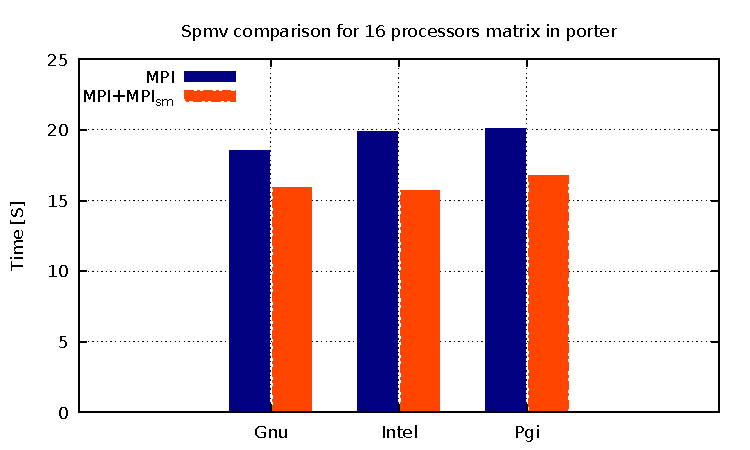
\includegraphics[page=1, width=0.95\linewidth]{Plots/HybridProgramming/spmvIndividual.pdf}
      \caption[]{Porter}
      \label{fig:HybridPorter}
    \end{subfigure}%
    \begin{subfigure}{.6\textwidth}
      \centering
      \hspace*{-1.5cm} 
      \includegraphics[page=2, width=0.95\linewidth]{Plots/HybridProgramming/spmvIndividual.pdf}
      \caption{Stout.}
      \label{fig:HybridStout}
    \end{subfigure}
    \begin{subfigure}{.6\textwidth}
      \centering
      \hspace*{-1.5cm} 
      \includegraphics[page=3, width=0.95\linewidth]{Plots/HybridProgramming/spmvIndividual.pdf}
      \caption[]{Dunkel.}
      \label{fig:HybridDunkel}
    \end{subfigure}%
    \begin{subfigure}{.6\textwidth}
      \centering
      \hspace*{-1.5cm} 
      \includegraphics[page=4, width=0.95\linewidth]{Plots/HybridProgramming/spmvIndividual.pdf}
      \caption{Koelsch.}
      \label{fig:HybridKoelsh}
    \end{subfigure}
\caption{MPI vs Hybrid $MPI+MPI_{Sm}$ SPMV comparison in individual systems.}
\label{fig:spmvIndividual}
\end{figure}


\medskip

The four systems used to obtain the results shown in Figure \ref{fig:spmvIndividual} were used together in the form of a four-node cluster, to evaluate the traditional and hybrid implementation of the SPMV kernel. Once again, three compilers were used in the evaluation. However this time, in addition of solving the previously matrix (16 processes), two other unstructured matrices were also tested: one divided among 32 processes (8 processes per node) and the other divided among 64 processes (16 processes per node). 


\begin{figure} [h!]
    \centering
    \captionsetup{justification=centering, singlelinecheck=false}
    \begin{subfigure}{.6\textwidth}
      \centering
      \hspace*{-1.5cm} 
      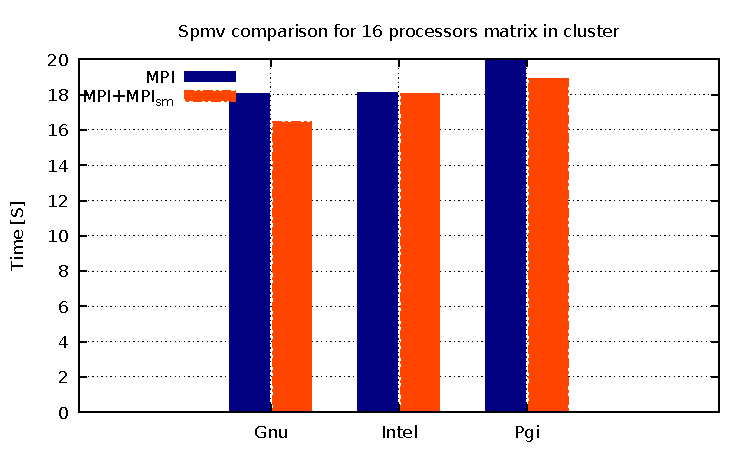
\includegraphics[page=1, width=0.95\linewidth]{Plots/HybridProgramming/spmvCluster.pdf}
      %\caption[]{Caption 1.}
      \label{fig:HybridPorter}
    \end{subfigure}%
    \begin{subfigure}{.6\textwidth}
      \centering
      \hspace*{-1.5cm} 
      \includegraphics[page=2, width=0.95\linewidth]{Plots/HybridProgramming/spmvCluster.pdf}
      %\caption{Caption 2.}
      \label{fig:HybridStout}
    \end{subfigure}
    \begin{subfigure}{.6\textwidth}
      \centering
      \hspace*{-1.5cm} 
      \includegraphics[page=3, width=0.95\linewidth]{Plots/HybridProgramming/spmvCluster.pdf}
      %\caption[]{Caption 3.}
      \label{fig:HybridDunkel}
    \end{subfigure}
\caption{MPI vs Hybrid $MPI+MPI_{Sm}$ SPMV comparison in 4-node cluster.}
\label{fig:spmvCluster4}
\end{figure}


\medskip

Figure \ref{fig:spmvCluster4} present the results obtained in the four-node cluster. Once again the hybrid version of the SPMV kernel shows different degrees of performance improvement with respect to its traditional counterpart, although the magnitude of performance improvement seems to vary depending on the matrix.

\medskip

To verify the results obtained in the 4-node cluster, the comparison of the three matrices was also done in 4 nodes of the Blue Waters supercomputer. However this test was only performed using the GNU compiler. Figure \ref{fig:spmvClusteBW} present this results. Once again, the hybrid version of the SPMV kernel always outperform the traditional one.

\medskip


\begin{figure} [h!]
    \centering
    \captionsetup{justification=centering, singlelinecheck=false}
    \begin{subfigure}{.6\textwidth}
      \centering
      \hspace*{-1.5cm} 
      \includegraphics[page=4, width=0.95\linewidth]{Plots/HybridProgramming/spmvCluster.pdf}
      %\caption[]{Blue Waters}
      \label{fig:HybridPorter}
    \end{subfigure}%
\caption{MPI vs Hybrid $MPI+MPI_{Sm}$ SPMV comparison in 4 Blue Waters nodes using the Gnu Compiler.}
\label{fig:spmvClusteBW}
\end{figure}




\subsection*{Summary}

The sparse matrix-vector multiplication represented by Equation \ref{eq:spmv} was used to compare a traditional (non-hybrid) parallel implementation with a hybrid one in which the \emph{v} vector was allocated using shared memory, effectively given access to it to all the processes co-existing in a node. Although the memory footprint was not changed, a reduction in the amount of communication required by the algorithm produce an increment of performance.


         % for SECTION 5    in "hybrid_programing.tex"
%\include{concl}                    % for CONCLUSION   in "concl.tex"


\bibliographystyle{plain}
\bibliography{references}
%\nocite{*}

%%%%%%%%%%%%%%%%%%%%%%%%%%%%%%%%%%%%%%%%%%%%%%%%%%%%%%%%%%%%%%%%%%%%%%%%%%%%%%%
\end{document}
